% Standalone TikZ source for the Sophia data-flow / template-generation diagram.
% Shows: Ariadne CTI graph -> Sophia templates (.docx authoring,
% template language, Cypher binding) -> data curation pipeline ->
% Alpaca-format IFT triples for Glaukopis training.
%
% Compile with: pdflatex glaukopis_sophia_flow.tex
% Render PNG:   pdftoppm -r 300 glaukopis_sophia_flow.pdf glaukopis_sophia_flow -png
\documentclass[tikz,border=6pt]{standalone}
\usepackage[T1]{fontenc}
\usetikzlibrary{arrows.meta,positioning,fit,backgrounds,calc,shapes.geometric}

\begin{document}
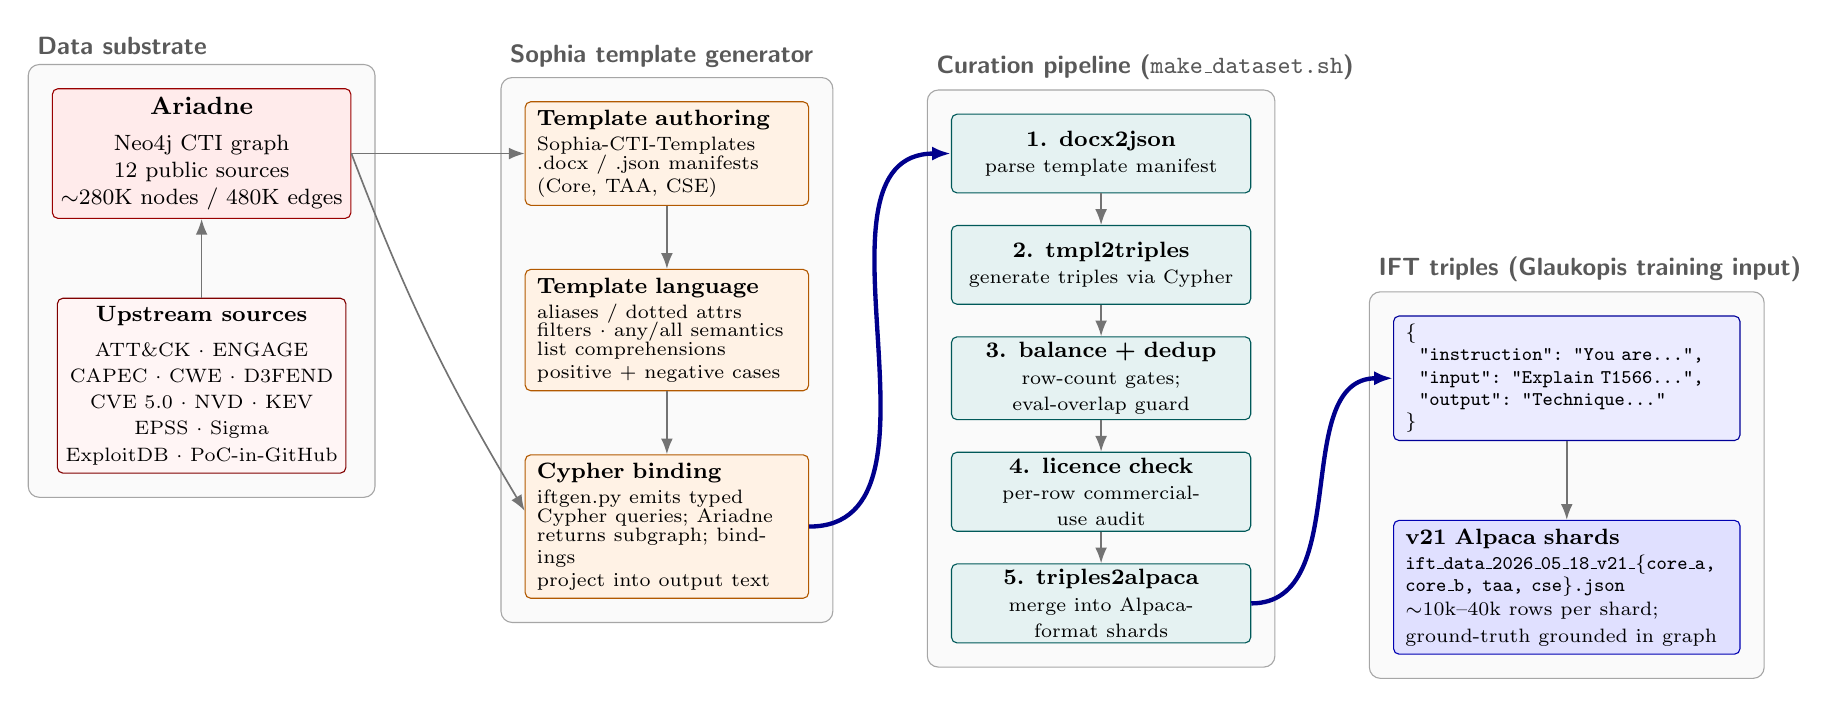
\begin{tikzpicture}[
    font=\rmfamily\small,
    >={Latex[length=2.2mm]},
    node distance=4mm and 6mm,
    src/.style       ={rectangle, rounded corners=2pt, draw=red!60!black, fill=red!8,
                       minimum width=36mm, minimum height=14mm, align=center, inner sep=3pt},
    tmpl/.style      ={rectangle, rounded corners=2pt, draw=orange!70!black, fill=orange!10,
                       minimum width=36mm, minimum height=11mm, align=left, inner sep=3pt,
                       font=\rmfamily\footnotesize, text width=33mm},
    pstep/.style      ={rectangle, rounded corners=2pt, draw=teal!70!black, fill=teal!10,
                       minimum width=38mm, minimum height=10mm, align=center, inner sep=2pt,
                       font=\rmfamily\footnotesize, text width=35mm},
    oblock/.style       ={rectangle, rounded corners=2pt, draw=blue!60!black, fill=blue!8,
                       minimum width=44mm, minimum height=14mm, align=left, inner sep=3pt,
                       font=\rmfamily\scriptsize\ttfamily, text width=41mm},
    grp/.style       ={rectangle, rounded corners=4pt, draw=black!35, fill=black!2,
                       inner sep=3mm},
    grptitle/.style  ={font=\rmfamily\bfseries\footnotesize, text=black!65},
    arr/.style       ={-{Latex[length=2mm]}, semithick, black!55},
    arrth/.style     ={-{Latex[length=2.4mm]}, line width=0.55mm, blue!55!black},
]

% =========================================
% Column 1: Ariadne CTI knowledge graph
% =========================================
\node[src] (ariadne)
   {\textbf{Ariadne}\\[0.5ex]\footnotesize Neo4j CTI graph\\[-0.3ex]\footnotesize 12 public sources\\[-0.3ex]\footnotesize $\sim$280K nodes / 480K edges};

\node[src, below=10mm of ariadne, fill=red!4, draw=red!50!black] (sources)
   {\footnotesize\textbf{Upstream sources}\\[0.4ex]
    \scriptsize ATT\&CK $\cdot$ ENGAGE\\[-0.4ex]
    \scriptsize CAPEC $\cdot$ CWE $\cdot$ D3FEND\\[-0.4ex]
    \scriptsize CVE 5.0 $\cdot$ NVD $\cdot$ KEV\\[-0.4ex]
    \scriptsize EPSS $\cdot$ Sigma\\[-0.4ex]
    \scriptsize ExploitDB $\cdot$ PoC-in-GitHub};
\draw[arr] (sources.north) -- (ariadne.south);

\begin{pgfonlayer}{background}
  \node[grp, fit=(ariadne)(sources)] (gA) {};
\end{pgfonlayer}
\node[grptitle, above=0mm of gA.north west, anchor=south west]
   {\sffamily\bfseries\small Data substrate};

% =========================================
% Column 2: Template authoring
% =========================================
\node[tmpl, right=22mm of ariadne.east, anchor=west] (auth)
   {\textbf{Template authoring}\\[0.3ex]
    \scriptsize Sophia-CTI-Templates\\[-0.4ex]
    \scriptsize .docx / .json manifests\\[-0.4ex]
    \scriptsize (Core, TAA, CSE)};

\node[tmpl, below=8mm of auth.south, anchor=north] (lang)
   {\textbf{Template language}\\[0.3ex]
    \scriptsize aliases / dotted attrs\\[-0.4ex]
    \scriptsize filters $\cdot$ any/all semantics\\[-0.4ex]
    \scriptsize list comprehensions\\[-0.4ex]
    \scriptsize positive + negative cases};

\node[tmpl, below=8mm of lang.south, anchor=north] (cypher)
   {\textbf{Cypher binding}\\[0.3ex]
    \scriptsize iftgen.py emits typed\\[-0.4ex]
    \scriptsize Cypher queries; Ariadne\\[-0.4ex]
    \scriptsize returns subgraph; bindings\\[-0.4ex]
    \scriptsize project into output text};

\begin{pgfonlayer}{background}
  \node[grp, fit=(auth)(lang)(cypher)] (gT) {};
\end{pgfonlayer}
\node[grptitle, above=0mm of gT.north west, anchor=south west]
   {\sffamily\bfseries\small Sophia template generator};

% Edges: Ariadne feeds the Cypher binding step
\draw[arr] (ariadne.east) -- ($(auth.west)+(0,0)$);
\draw[arr] (ariadne.east) to[bend right=5] ($(cypher.west)+(0,2mm)$);

% Auth -> lang -> cypher chain
\draw[arr] (auth.south) -- (lang.north);
\draw[arr] (lang.south) -- (cypher.north);

% =========================================
% Column 3: Pipeline curation steps
% =========================================
\node[pstep, right=18mm of auth.east, anchor=west] (s1)
   {\textbf{1. docx2json}\\[0pt]\scriptsize parse template manifest};
\node[pstep, below=4mm of s1.south, anchor=north] (s2)
   {\textbf{2. tmpl2triples}\\[0pt]\scriptsize generate triples via Cypher};
\node[pstep, below=4mm of s2.south, anchor=north] (s3)
   {\textbf{3. balance + dedup}\\[0pt]\scriptsize row-count gates; eval-overlap guard};
\node[pstep, below=4mm of s3.south, anchor=north] (s4)
   {\textbf{4. licence check}\\[0pt]\scriptsize per-row commercial-use audit};
\node[pstep, below=4mm of s4.south, anchor=north] (s5)
   {\textbf{5. triples2alpaca}\\[0pt]\scriptsize merge into Alpaca-format shards};

% Edges from Sophia generator to step 1
\draw[arrth] (cypher.east) to[out=0,in=180] (s1.west);

% chain the 5 steps
\draw[arr] (s1.south) -- (s2.north);
\draw[arr] (s2.south) -- (s3.north);
\draw[arr] (s3.south) -- (s4.north);
\draw[arr] (s4.south) -- (s5.north);

\begin{pgfonlayer}{background}
  \node[grp, fit=(s1)(s5)] (gP) {};
\end{pgfonlayer}
\node[grptitle, above=0mm of gP.north west, anchor=south west]
   {\sffamily\bfseries\small Curation pipeline (\texttt{make\_dataset.sh})};

% =========================================
% Column 4: IFT triples (output)
% =========================================
\node[oblock, right=18mm of s3.east, anchor=west] (alpaca)
   {\{ \\
    \ \ "instruction": "You are\ldots", \\
    \ \ "input": "Explain T1566\ldots", \\
    \ \ "output": "Technique\ldots" \\
    \}};

\node[oblock, below=10mm of alpaca.south, anchor=north,
      font=\rmfamily\footnotesize, draw=blue!70!black, fill=blue!12, text width=41mm]
   (shards)
   {\textbf{v21 Alpaca shards}\\[0.3ex]
    \scriptsize\ttfamily ift\_data\_2026\_05\_18\_v21\_\{core\_a, core\_b, taa, cse\}.json\\[0.3ex]
    \scriptsize\rmfamily{$\sim$10k--40k rows per shard;}\\
    \scriptsize\rmfamily{ground-truth grounded in graph}};

% Edge from step 5 to alpaca
\draw[arrth] (s5.east) to[out=0,in=180] (alpaca.west);
\draw[arr] (alpaca.south) -- (shards.north);

\begin{pgfonlayer}{background}
  \node[grp, fit=(alpaca)(shards)] (gO) {};
\end{pgfonlayer}
\node[grptitle, above=0mm of gO.north west, anchor=south west]
   {\sffamily\bfseries\small IFT triples (Glaukopis training input)};

\end{tikzpicture}
\end{document}
